\documentclass{article}

\usepackage{xcolor}
\usepackage{hyperref}
\definecolor{COLOR_MEAN}{HTML}{f0f0f0}
\definecolor{LINK_COLOR}{HTML}{636EFA}
\hypersetup{
	colorlinks=true,
	linkcolor=LINK_COLOR,
	urlcolor=LINK_COLOR,
	citecolor=LINK_COLOR,
}

\usepackage{array}
\usepackage{colortbl}

% if you need to pass options to natbib, use, e.g.:
%     \PassOptionsToPackage{numbers, compress}{natbib}
% before loading neurips_2024


% ready for submission
%\usepackage{neurips_2024}


% to compile a preprint version, e.g., for submission to arXiv, add add the
% [preprint] option:
% \usepackage[preprint]{neurips_2024}


% to compile a camera-ready version, add the [final] option, e.g.:
\usepackage[final]{neurips_2024}


% to avoid loading the natbib package, add option nonatbib:
%    \usepackage[nonatbib]{neurips_2024}


\usepackage[utf8]{inputenc} % allow utf-8 input
\usepackage[T1]{fontenc}    % use 8-bit T1 fonts
\usepackage{hyperref}       % hyperlinks
\usepackage{url}            % simple URL typesetting
\usepackage{booktabs}       % professional-quality tables
\usepackage{amsfonts}       % blackboard math symbols
\usepackage{nicefrac}       % compact symbols for 1/2, etc.
\usepackage{microtype}      % microtypography
\usepackage{xcolor}         % colors
\usepackage{tabularx}
\usepackage{booktabs}
\usepackage{amsmath}
\usepackage{listings}
\usepackage{tikz}

\title{MH4320 Assignment 5}


% The \author macro works with any number of authors. There are two commands
% used to separate the names and addresses of multiple authors: \And and \AND.
%
% Using \And between authors leaves it to LaTeX to determine where to break the
% lines. Using \AND forces a line break at that point. So, if LaTeX puts 3 of 4
% authors names on the first line, and the last on the second line, try using
% \AND instead of \And before the third author name.


\author{%
	Pu Fanyi \\
	College of Computing and Data Science\\
	Nanyang Technological University\\
	Singapore 639798 \\
	\texttt{FPU001@e.ntu.edu.sg} \\
}

\usepackage{graphicx}

\begin{document}
	
	
	\maketitle	
	
	\section{Subgame Perfect Equilibria}

    \subsection{Subgame Perfect Equilibria in Pure Strategies}

    For the subgame:

    \begin{center}
        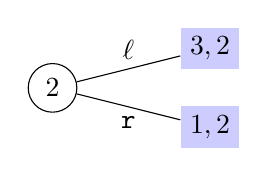
\begin{tikzpicture}[scale=2]
            % Nodes
            % \node[circle, draw] (n1) at (0,0) {1};
            \node[circle, draw] (n2) at (1,0) {2};
            \node[rectangle, fill=blue!20] (n3) at (2,0.25) {\(3,2\)};
            \node[rectangle, fill=blue!20] (n4) at (2,-0.25) {\(1,2\)};
            % \node[rectangle, fill=blue!20] (n5) at (0,-1) {\(2,0\)};
            
            % Edges
            % \draw (n1) -- (n2) node[midway, above] {\(U\)};
            % \draw (n1) -- (n5) node[midway, left] {\(D\)};
            \draw (n2) -- (n3) node[midway, above] {\(\ell\)};
            \draw (n2) -- (n4) node[midway, below] {\(\mathtt{r}\)};
        \end{tikzpicture}
    \end{center}

    There is no difference for player 2 to play $\ell$ or $\mathtt{r}$.

    For the subgame:
    
    \begin{center}
        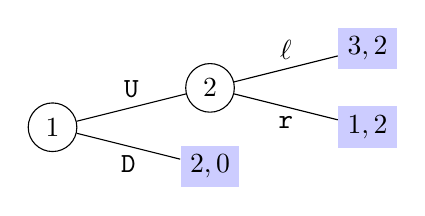
\begin{tikzpicture}[scale=2]
            % Nodes
            \node[circle, draw] (n1) at (0,-0.25) {1};
            \node[circle, draw] (n2) at (1,0) {2};
            \node[rectangle, fill=blue!20] (n3) at (2,0.25) {\(3,2\)};
            \node[rectangle, fill=blue!20] (n4) at (2,-0.25) {\(1,2\)};
            \node[rectangle, fill=blue!20] (n5) at (1,-0.5) {\(2,0\)};
            
            % Edges
            \draw (n1) -- (n2) node[midway, above] {\(\mathtt{U}\)};
            \draw (n1) -- (n5) node[midway, below] {\(\mathtt{D}\)};
            \draw (n2) -- (n3) node[midway, above] {\(\ell\)};
            \draw (n2) -- (n4) node[midway, below] {\(\mathtt{r}\)};
        \end{tikzpicture}
    \end{center}

    We have:

    \begin{center}
    \begin{tabular}{c|c c}
    & $\ell$ & $\mathtt{r}$ \\\hline
    $\mathtt{U}$ & $3,2$ & $1,2$ \\
    $\mathtt{D}$ & $2,0$ & $2,0$
    \end{tabular}
    \end{center}

    The pure NEs are $(\mathtt{U}, \ell)$ and $(\mathtt{D}, \mathtt{r})$.

    \subsection{Subgame Perfect Equilibria in Mixed Strategies}

    For player 1 and 2 both play pure strategy, the NEs are $(\mathtt{U}, \ell)$ and $(\mathtt{D}, \mathtt{r})$.

    There is no difference for play 2 to choose between $\ell$ and $\texttt{r}$. So let player 2 plays $(p_2, 1-p_2)$.

    When $p_2>\frac{1}{2}$, $\mathtt{U}$ is the best response, as $3p_2+(1-p_2)=1+2p_2>2$. So player 1 should play $\mathtt{U}$.

    When $p_2<\frac{1}{2}$, $\mathtt{D}$ is the best response, as $3p_2+(1-p_2)=1+2p_2<2$. So player 1 should play $\mathtt{D}$.

    When $p_2=\frac{1}{2}$, there is no difference for player 1 to choose between $\mathtt{U}$ and $\mathtt{D}$. So player 1 can play $(p_1, 1-p_1)$ for any $p_1\in[0, 1]$.

    So all SPEs in mixed strategies are:

    $$
    \left\{\left[(p_1, 1-p_1), \left(\frac{1}{2}, \frac{1}{2}\right)\right]: p_1\in[0, 1]\right\}
        \cup\left\{\left[(1, 0), \left(p_2, 1-p_2\right)\right]: p_2>\frac{1}{2}\right\}\left\{\left[(0, 1), \left(p_2, 1-p_2\right)\right]: p_2<\frac{1}{2}\right\}
    $$

    \section{Incomplete Information Extensive-Form Games}

    \subsection{Strategic-Form Representation}

    \begin{center}
    \begin{tabular}{c|c c}
    & $\mathtt{U}$ & $\mathtt{D}$ \\\hline
    $\mathtt{L}, \ell$ & $3,3$ & $0, 2$ \\
    $\mathtt{L}, \mathtt{r}$ & $2,0$ & $2,2$ \\
    $\mathtt{R}, \mathtt{*}$ & $\frac{5}{2}, \frac{5}{2}$ & $\frac{5}{2}, \frac{5}{2}$ \\
    \end{tabular}
    \end{center}

    \subsection{Number of Subgames}

    There are 2 subgames:

    \begin{enumerate}
        \item The first subgame is the whole game, the starting node is $1$.
            \begin{center}
        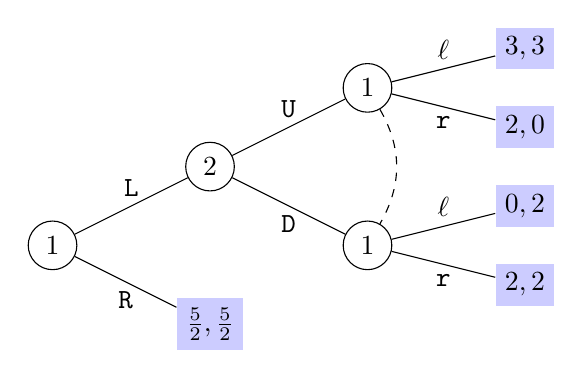
\begin{tikzpicture}[scale=2]
            % Nodes
            \node[circle, draw] (n1) at (0,0.25) {2};
            \node[circle, draw] (n2) at (1,0.75) {1};
            \node[circle, draw] (n3) at (1,-0.25) {1};
            \node[rectangle, fill=blue!20] (n4) at (2,1) {\(3, 3\)};
            \node[rectangle, fill=blue!20] (n5) at (2,0.5) {\(2,0\)};
            \node[rectangle, fill=blue!20] (n6) at (2,0) {\(0,2\)};
            \node[rectangle, fill=blue!20] (n7) at (2,-.5) {\(2,2\)};
            \node[circle, draw] (n8) at (-1,-0.25) {1};
            \node[rectangle, fill=blue!20] (n9) at (0,-.75) {\(\frac{5}{2}, \frac{5}{2}\)};
            
            % Edges
            \draw (n1) -- (n2) node[midway, above] {\(\mathtt{U}\)};
            \draw (n1) -- (n3) node[midway, below] {\(\mathtt{D}\)};
            \draw (n2) -- (n4) node[midway, above] {\(\ell\)};
            \draw (n2) -- (n5) node[midway, below] {\(\mathtt{r}\)};
            \draw (n3) -- (n6) node[midway, above] {\(\ell\)};
            \draw (n3) -- (n7) node[midway, below] {\(\mathtt{r}\)};
            \draw (n8) -- (n1) node[midway, above] {\(\mathtt{L}\)};
            \draw (n8) -- (n9) node[midway, below] {\(\mathtt{R}\)};

            \draw[dashed] (n2) to [bend left] (n3);
        \end{tikzpicture}
    \end{center}
        \item The second subgame is the game after player 1 playing $\mathtt{L}$, the starting node is 2.    \begin{center}
        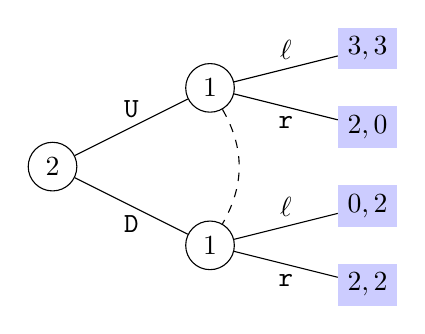
\begin{tikzpicture}[scale=2]
            % Nodes
            \node[circle, draw] (n1) at (0,0.25) {2};
            \node[circle, draw] (n2) at (1,0.75) {1};
            \node[circle, draw] (n3) at (1,-0.25) {1};
            \node[rectangle, fill=blue!20] (n4) at (2,1) {\(3, 3\)};
            \node[rectangle, fill=blue!20] (n5) at (2,0.5) {\(2,0\)};
            \node[rectangle, fill=blue!20] (n6) at (2,0) {\(0,2\)};
            \node[rectangle, fill=blue!20] (n7) at (2,-.5) {\(2,2\)};
            
            % Edges
            \draw (n1) -- (n2) node[midway, above] {\(\mathtt{U}\)};
            \draw (n1) -- (n3) node[midway, below] {\(\mathtt{D}\)};
            \draw (n2) -- (n4) node[midway, above] {\(\ell\)};
            \draw (n2) -- (n5) node[midway, below] {\(\mathtt{r}\)};
            \draw (n3) -- (n6) node[midway, above] {\(\ell\)};
            \draw (n3) -- (n7) node[midway, below] {\(\mathtt{r}\)};

            \draw[dashed] (n2) to [bend left] (n3);
        \end{tikzpicture}
    \end{center}
    \end{enumerate}

    \subsection{Subgame Perfect Equilibria}

    Let's see the subgame first:

    \begin{center}
        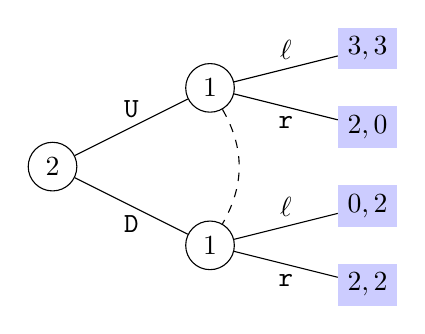
\begin{tikzpicture}[scale=2]
            % Nodes
            \node[circle, draw] (n1) at (0,0.25) {2};
            \node[circle, draw] (n2) at (1,0.75) {1};
            \node[circle, draw] (n3) at (1,-0.25) {1};
            \node[rectangle, fill=blue!20] (n4) at (2,1) {\(3, 3\)};
            \node[rectangle, fill=blue!20] (n5) at (2,0.5) {\(2,0\)};
            \node[rectangle, fill=blue!20] (n6) at (2,0) {\(0,2\)};
            \node[rectangle, fill=blue!20] (n7) at (2,-.5) {\(2,2\)};
            
            % Edges
            \draw (n1) -- (n2) node[midway, above] {\(\mathtt{U}\)};
            \draw (n1) -- (n3) node[midway, below] {\(\mathtt{D}\)};
            \draw (n2) -- (n4) node[midway, above] {\(\ell\)};
            \draw (n2) -- (n5) node[midway, below] {\(\mathtt{r}\)};
            \draw (n3) -- (n6) node[midway, above] {\(\ell\)};
            \draw (n3) -- (n7) node[midway, below] {\(\mathtt{r}\)};

            \draw[dashed] (n2) to [bend left] (n3);
        \end{tikzpicture}
    \end{center}

    We can convert it to strategic form:

    \begin{center}
    \begin{tabular}{c|c c}
    & $\mathtt{U}$ & $\mathtt{D}$ \\\hline
    $\ell$ & $3,3$ & $0, 2$ \\
    $\mathtt{r}$ & $2,0$ & $2,2$ \\
    \end{tabular}
    \end{center}

    The pure NEs for the subgame are: $(\ell, \mathtt{U}), (\mathtt{r}, \mathtt{D})$, the utilities for each NEs are $(3, 3), (2, 2)$. And there is a mixed NE $\left[\left(\frac{2}{3}, \frac{1}{3}\right), \left(\frac{2}{3}, \frac{1}{3}\right)\right]$, the utilities are $(2, 2)$.

    So when we perform backward induction to the whole game:

    \begin{center}
        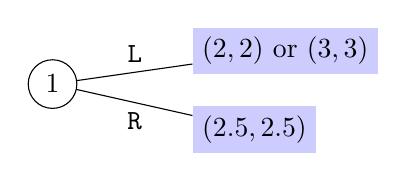
\begin{tikzpicture}[scale=2]
            % Nodes
            \node[rectangle, fill=blue!20, anchor=north west] (n1) at (0,0.25) {$(2, 2)$ or $(3, 3)$};
            \node[circle, draw, anchor=north west] (n8) at (-1,0) {1};
            \node[rectangle, fill=blue!20, anchor=north west] (n9) at (0,-0.25) {\(\left(2.5, 2.5\right)\)};
            
            % Edges
            \draw (n8) -- (n1) node[midway, above] {\(\mathtt{L}\)};
            \draw (n8) -- (n9) node[midway, below] {\(\mathtt{R}\)};
        \end{tikzpicture}
    \end{center}

    For the NE $2, 2$, player 1 will change to $\mathtt{R}$, and for $3, 3$, player 1 will choose $\mathtt{L}$.

    So the SPEs are:

    $$
    \left\{\left[\mathtt{L}, \ell, \mathtt{U}\right], \left[\mathtt{R}, \mathtt{D}, \mathtt{r}\right], \left[\mathtt{R}, \frac{2}{3}\mathtt{U}+\frac{1}{3}\mathtt{D}, \frac{2}{3}\ell+\frac{1}{3}\mathtt{r}\right]\right\}
    $$

    \section{War of Attrition}

    For the second stage, we have the subgame:

    $$
    -c + \begin{array}{c|c c}
    & \mathtt{f_2} & \mathtt{q_2} \\\hline
    \mathtt{F_2} & -c, -c & v, 0\\
    \mathtt{Q_2} & 0, v & 0, 0
    \end{array}
    $$

    For the table, there are $2$ pure NEs: $(\mathtt{F_2}, \mathtt{q_2}), (\mathtt{Q_2, f_2})$, with payoff $(v, 0), (0, v)$ separately.

    For mixed strategy, let $P_1$ plays $(p_1, 1-p_1)$, $P_2$ plays $(q_2, 1-q_2)$.

    We have:
    $$
    \begin{cases}
        -cq_1+v(1-q_1)=0\\
        -cq_2+v(1-q_2)=0
    \end{cases}
    $$

    So
    $$
    q_1=q_2=\frac{v}{c+v}
    $$

    So the mixed strategy is
    $$
    \left[\left(\frac{v}{c+v}\mathtt{F_2}, \frac{c}{c+v}\mathtt{Q_2}\right), \left(\frac{v}{c+v}\mathtt{f_2}, \frac{c}{c+v}\mathtt{q_2}\right)\right]
    $$

    Now, let's consider the first stage.
    
    If we take $(\mathtt{F_2}, \mathtt{q_2})$ as NE, We have:
    $$
    \begin{array}{c|c c}
    & \mathtt{f_1} & \mathtt{q_1} \\\hline
    \mathtt{F_1} & v-c, -c & v, 0\\
    \mathtt{Q_1} & 0, v & 0, 0
    \end{array}
    $$

    It is easy to find the pure NEs $(\mathtt{F_1}, \mathtt{q_1}), (\mathtt{Q_1}, \mathtt{f_1})$ and mixed NE $\left(\frac{v}{c+v}\mathtt{F_1}+\frac{c}{c+v}\mathtt{Q_1}, \frac{v}{c}\mathtt{f_1}+\frac{c-v}{c}\mathtt{q_1}\right)$.

    So the NEs are:

    $$
    \left\{\left[\left(\mathtt{F_1}, \mathtt{F_2}\right), \left(\mathtt{q_1}, \mathtt{q_2}\right)\right], \left[\left(\mathtt{Q_1}, \mathtt{F_2}\right), \left(\mathtt{f_1}, \mathtt{q_2}\right)\right], \left[\left(\frac{v}{c+v}\mathtt{F_1}+\frac{c}{c+v}\mathtt{Q_1}, \mathtt{F_2}\right), \left(\frac{v}{c}\mathtt{f_1}+\frac{c-v}{c}\mathtt{q_1}, \mathtt{q_2}\right)\right]\right\}
    $$

    If we take $(\mathtt{Q_2}, \mathtt{f_2})$ as NE, We have:
    $$
    \begin{array}{c|c c}
    & \mathtt{f_1} & \mathtt{q_1} \\\hline
    \mathtt{F_1} & -c, v-c & v, 0\\
    \mathtt{Q_1} & 0, v & 0, 0
    \end{array}
    $$

    It is easy to find the pure NEs $(\mathtt{F_1}, \mathtt{q_1}), (\mathtt{Q_1}, \mathtt{f_1})$ and mixed NE $\left(\frac{v}{c}\mathtt{F_1}+\frac{c-v}{c}\mathtt{Q_1}, \frac{v}{c+v}\mathtt{f_1}+\frac{c}{c+v}\mathtt{q_1}\right)$.

    So the NEs are:

    $$
    \left\{
    \left[\left(\mathtt{F_1}, \mathtt{Q_2}\right),\left(\mathtt{q_1}, \mathtt{f_2}\right)\right], \left[\left(\mathtt{Q_1}, \mathtt{Q_2}\right), \left(\mathtt{f_1}, \mathtt{f_2}\right)\right], 
    \left[\left(\frac{v}{c}\mathtt{F_1}+\frac{c-v}{c}\mathtt{Q_1}, \mathtt{Q_2}\right), \left(\frac{v}{c+v}\mathtt{f_1}+\frac{c}{c+v}\mathtt{q_1}, \mathtt{f_2}\right)\right]\right\}
    $$


    \section{Alice and Bob}

    \subsection{Extensive and Strategic Form of the Game}

    \subsubsection{Extensive Form}
    
    \begin{center}
        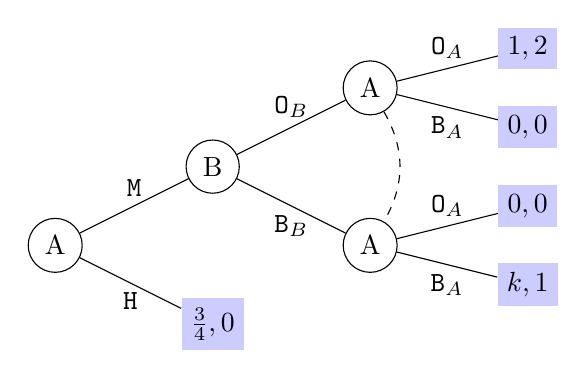
\begin{tikzpicture}[scale=2]
            % Nodes
            \node[circle, draw] (n1) at (0,0.25) {B};
            \node[circle, draw] (n2) at (1,0.75) {A};
            \node[circle, draw] (n3) at (1,-0.25) {A};
            \node[rectangle, fill=blue!20] (n4) at (2,1) {\(1,2\)};
            \node[rectangle, fill=blue!20] (n5) at (2,0.5) {\(0,0\)};
            \node[rectangle, fill=blue!20] (n6) at (2,0) {\(0,0\)};
            \node[rectangle, fill=blue!20] (n7) at (2,-.5) {\(k,1\)};
            \node[circle, draw] (n8) at (-1,-0.25) {A};
            \node[rectangle, fill=blue!20] (n9) at (0,-.75) {\(\frac{3}{4}, 0\)};
            
            % Edges
            \draw (n1) -- (n2) node[midway, above] {\(\mathtt{O}_B\)};
            \draw (n1) -- (n3) node[midway, below] {\(\mathtt{B}_B\)};
            \draw (n2) -- (n4) node[midway, above] {\(\mathtt{O}_A\)};
            \draw (n2) -- (n5) node[midway, below] {\(\mathtt{B}_A\)};
            \draw (n3) -- (n6) node[midway, above] {\(\mathtt{O}_A\)};
            \draw (n3) -- (n7) node[midway, below] {\(\mathtt{B}_A\)};
            \draw (n8) -- (n1) node[midway, above] {\(\mathtt{M}\)};
            \draw (n8) -- (n9) node[midway, below] {\(\mathtt{H}\)};

            \draw[dashed] (n2) to [bend left] (n3);
        \end{tikzpicture}
    \end{center}

    \subsubsection{Strategic Form}

    \begin{center}
    \begin{tabular}{c|c c}
    & $\mathtt{O}_B$ & $\mathtt{B}_B$ \\\hline
    $\mathtt{M}, \mathtt{O}_A$ & $1,2$ & $0, 0$ \\
    $\mathtt{M}, \mathtt{B}_A$ & $0,0$ & $k,1$ \\
    $\mathtt{H}, \mathtt{O}_A$ & $\frac{3}{4}, 0$ & $\frac{3}{4}, 0$ \\
    $\mathtt{H}, \mathtt{B}_A$ & $\frac{3}{4}, 0$ & $\frac{3}{4}, 0$ \\
    \end{tabular}
    \end{center}

    \subsection{Values of k}

    For the subgame:
    \begin{center}
        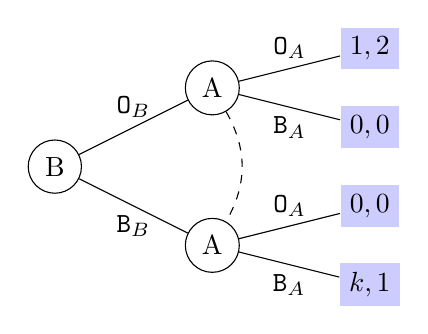
\begin{tikzpicture}[scale=2]
            % Nodes
            \node[circle, draw] (n1) at (0,0.25) {B};
            \node[circle, draw] (n2) at (1,0.75) {A};
            \node[circle, draw] (n3) at (1,-0.25) {A};
            \node[rectangle, fill=blue!20] (n4) at (2,1) {\(1,2\)};
            \node[rectangle, fill=blue!20] (n5) at (2,0.5) {\(0,0\)};
            \node[rectangle, fill=blue!20] (n6) at (2,0) {\(0,0\)};
            \node[rectangle, fill=blue!20] (n7) at (2,-.5) {\(k,1\)};
            
            % Edges
            \draw (n1) -- (n2) node[midway, above] {\(\mathtt{O}_B\)};
            \draw (n1) -- (n3) node[midway, below] {\(\mathtt{B}_B\)};
            \draw (n2) -- (n4) node[midway, above] {\(\mathtt{O}_A\)};
            \draw (n2) -- (n5) node[midway, below] {\(\mathtt{B}_A\)};
            \draw (n3) -- (n6) node[midway, above] {\(\mathtt{O}_A\)};
            \draw (n3) -- (n7) node[midway, below] {\(\mathtt{B}_A\)};

            \draw[dashed] (n2) to [bend left] (n3);
        \end{tikzpicture}
    \end{center}

    We can write it in strategic form:

    \begin{center}
    \begin{tabular}{c|c c}
    & $\mathtt{O}_B$ & $\mathtt{B}_B$ \\\hline
    $\mathtt{O}_A$ & $1,2$ & $0,0$ \\
    $\mathtt{B}_A$ & $0,0$ & $k,1$
    \end{tabular}
    \end{center}

    There are $2$ pure NEs $(\mathtt{O}_A, \mathtt{O}_B), (\mathtt{B}_A, \mathtt{B}_B)$ with outcome $(1, 2)$ and $(k, 1)$.

    For mixed strategy, let $A$ plays $(p_A, 1-p_A)$, $B$ plays $(p_B, 1-p_B)$.

    We have:
    $$
    \begin{cases}
        2p_A=1-p_A\\
        p_B=k(1-p_B)
    \end{cases}
    $$

    So
    $$
    \begin{cases}
        p_A=\frac{1}{3}\\
        p_B=\frac{k}{1+k}
    \end{cases}
    $$

    So the utility for Alice is:
    $$
    \frac{1}{3}\cdot\frac{k}{1+k}+\frac{2}{3}\cdot k\cdot\frac{1}{1+k}=\frac{k}{1+k}
    $$

    To make all the subgame-perfect equilibria involves Alice’s going to the movies, we should have:
    $$
    \begin{cases}
        1>\frac{3}{4}\\
        k>\frac{3}{4}\\
        \frac{k}{1+k}>\frac{3}{4}
    \end{cases}
    $$

    So $k>3$.
\end{document}